\section{Statechart diagrams} \label{sec:statechart}
Statechart diagrams are a useful way to get an overview over the lifetime of objects in the problem domain.
This section describes the state chart diagram of objects whose behaivour is both interesting and unique to the project.
Due to the nature of the application, it being very focused on basic \textit{create, read, update and delete} (CRUD) operations, there is not a lot of interesting activity going on in the way of state.
% Taniya: måske droppe "there is not a lot of interesting activity going on in the way of state." delen. Lyder mere som en personlig holdning. Eller misforstår jeg hvad der menes med sætningen?

\subsection{Approval Request}
The approval request is one of the most central concepts in the application.
When someone wants to create a new version of a document, they instantiate an approval request, which has a version object attached.
The change will have to be approved several times before it will actually be released.
When the change is approved, it will append the version to the document object. When the change is denied, it will simply sit as pending until it is reapproved.

% skal deny være en del af statechart eftersom vi har besluttet os at fjerne Approval denied event i en tidligere sektion? Man har ikke mulighed for at lave en Approval denial event, men man kan slette en approval og laver en ny approval

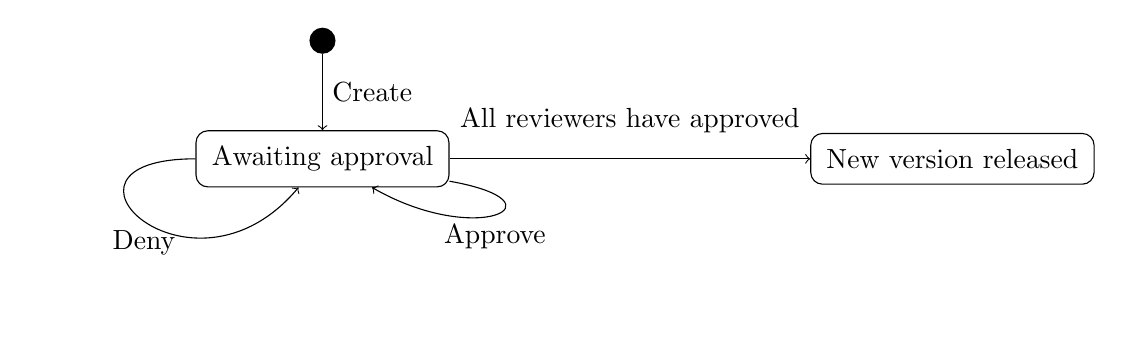
\begin{tikzpicture}[round/.style={rounded corners=1.5mm,minimum width=1cm,inner sep=2mm,above right,draw,align=left}]

	\node[circle, fill=black,minimum size=3pt] (start) {};
	\node[round] (await) [below of=start, node distance=1.5cm] {Awaiting approval};
	\path[->] (start) edge node[right] {Create} (await);
	\path[->] (await) edge [loop below, out=350, in=330, looseness=4] node {Approve} (await);
	\path[->] (await) edge [loop below, out=180, in=230, looseness=4] node {Deny} (await);
	\node[round] (approved) [right of=await, node distance=8cm] {New version released};
	\path[->] (await) edge node[above, yshift=0.2cm] {All reviewers have approved} (approved);

	%\draw[fill=white] circle[radius = 7pt, below of=approved, node distance=1cm];
	%\node[circle, fill=black,minimum size=3pt] (end) [below of=approved, node distance=1cm] {};


\end{tikzpicture}

\subsection{Department}
A department is an organisational unit, used to administrate which users are attached to which documents.
As such, you can create a department, add users to it, and add documents to it.
You can also remove both in the same way.
One of the most important functions of the department is the abillity for it to notify all the users which are attached to it of a new version of a document.

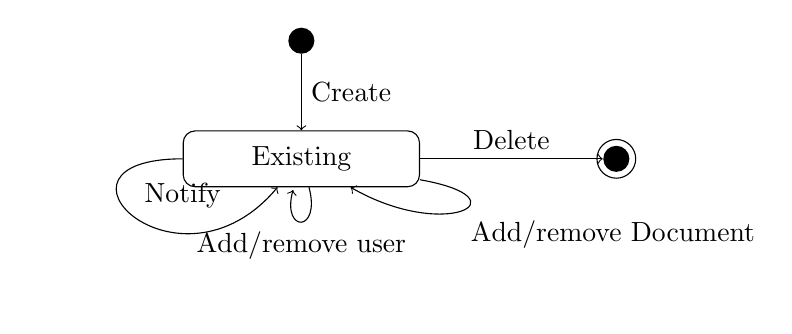
\begin{tikzpicture}[round/.style={rounded corners=1.5mm,minimum width=1cm,inner sep=2mm,above right,draw,align=left}]

	\node[circle, fill=black,minimum size=3pt] (start) {};
	\node[round, minimum width=3cm] (await) [below of=start, node distance=1.5cm] {Existing};
	\path[->] (start) edge node[right] {Create} (await);
	\path[->] (await) edge [loop below] node[auto] {Add/remove user} (await);
	\path[->] (await) edge [loop below, out=350, in=330, looseness=4] node[auto] {Add/remove Document} (await);
	\path[->] (await) edge [loop below, out=180, in=230, looseness=4] node[auto] {Notify} (await);

	\draw[fill=white] circle[radius = 7pt, right of=await, node distance=4cm];
	\node[circle, fill=black,minimum size=3pt] (end) [right of=await, node distance=4cm] {};
	\path[->] (await) edge node[above] {Delete} (end);


\end{tikzpicture}

\subsection{Version}
A version is another central concept in the application.
As mentioned before, the handbook consists of documents, and each document can have multiple versions.
And thus, after creation, version objects are supposed to be quite immutable once created, as to preserve the history of individual documents.

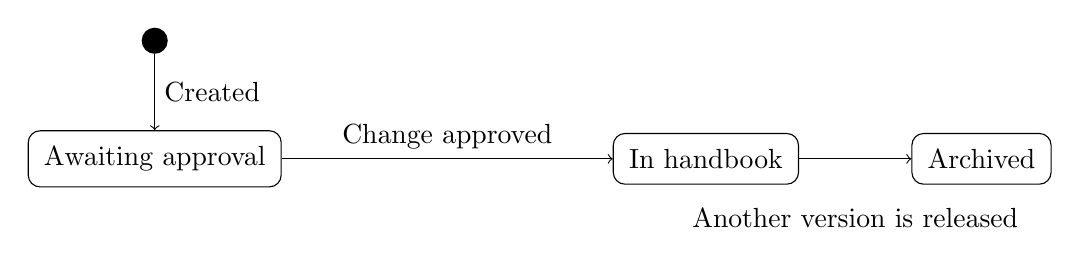
\begin{tikzpicture}[round/.style={rounded corners=1.5mm,minimum width=1cm,inner sep=2mm,above right,draw,align=left}]

	\node[circle, fill=black,minimum size=3pt] (start) {};
	\node[round] (await) [below of=start, node distance=1.5cm] {Awaiting approval};
	\path[->] (start) edge node[right] {Created} (await);
	\node[round] (approved) [right of=await, node distance=7cm] {In handbook};
	\path[->] (await) edge node[above] {Change approved} (approved);
	\node[round] (archived) [right of=approved, node distance=3.5cm] {Archived};
	\path[->] (approved) edge node[below, yshift=-0.5cm] {Another version is released} (archived);

	%\draw[fill=white] circle[radius = 7pt, below of=approved, node distance=1cm];
	%\node[circle, fill=black,minimum size=3pt] (end) [below of=approved, node distance=1cm] {};


\end{tikzpicture}

\section{Summary}

In this chapter the problem domain has been analysed where object oriented analysis principles were used regarding to the systematic selection of classes and events. The output is an event table representing relations between classes and events seen in \cref{fig:eventtable}.
Based on these relations between classes and events the structural relations between classes has been produced illustrating in a class diagram in \cref{fig:ClassDiagram}. The most significant behaviour for objects has been described and represented in statechart diagrams in \cref{sec:statechart}. The classes and the behaviour has been explored, it is therefore possible to examine how the actors interact with the system in the application domain in the next chapter.